\section{Background and Motivation}
\label{sec:motivation}
\begin{figure}[t]
\centering
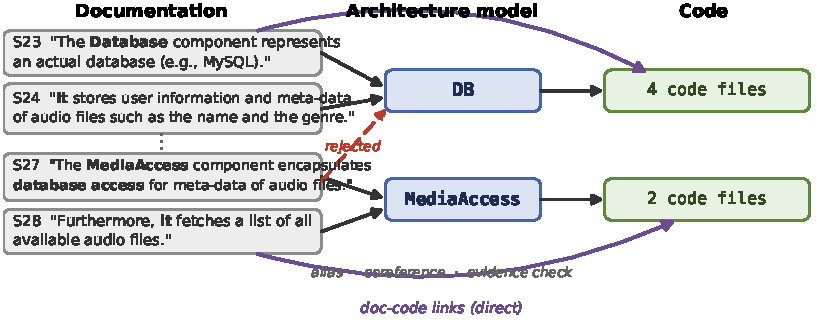
\includegraphics[width=\linewidth]{figures/jabref_trace_example}
% \caption{A simplified documentation-to-model-to-code trace link example.
% % Sentence~6 introduces the \texttt{gui} component under the alias ``UI''; Sentence~7
% % then refers to the same component by the pronoun ``it'' while mentioning ``preferences'' as
% % an ordinary word. Sentence~11 describes the \texttt{preferences} component, implemented under
% % \texttt{org/jabref/preferences/}. Each component maps to a code package (model-code); the purple
% % edges are the resulting direct doc-code links, and the dashed red edge is the false positive a
% % judge must reject.
% }
\Description{An example with documentation sentences on the left, architecture components in the middle, and code packages on the right. It shows correct trace links from the documentation to the gui and preferences components and to their code packages, plus one false positive link from a sentence mentioning preferences as an ordinary word.}
\label{fig:example}
\end{figure}

%SPEC style: short declaratives, one claim per sentence, low clause depth.
%SPEC framing: challenge-first -> consequence -> required capability / evaluation implication.
%SPEC thread: keep the JabRef running example across all subsections; reuse S6/S7/S11 consistently.
%SPEC scope: kp+jd merged = missed true link AND false positive from the same sentence; ev = misleading aggregate score from long-tailed link distribution.
%SPEC wording: prefer mention/refer/link/support; avoid surface; avoid inflated LLM language unless the text evidence supports it.
%SPEC metrics: do not call link-level \fone invalid; frame it as answering a different, size-weighted question that can hide component abandonment.
%SPEC numbers: keep only argument-carrying figures inline in motivation; trim secondary numbers from the rhetorical foreground.
%SPEC levels: distinguish doc-model from doc-code explicitly; reserve component for architecture level and package/file links for expansion level.
%SPEC solution-boundary: motivation = the disease, approach = the cure. Light capability hints allowed (what the task demands); no module names, no approach framing.

\subsection{Motivating Example}
A trace link connects a documentation sentence to an architecture component (doc-model) or to code (doc-code).
\autoref{fig:example} shows this setup on JabRef, a reference manager software.
Sentence~11 describes the \texttt{preferences} component, which maps to the code package \texttt{org/jabref/preferences/}.
Sentence~7 describes the \texttt{gui} component, but it also contains the word ``preferences.''
That one sentence already shows two problems that make automatic recovery hard.
A reference uses no component name, and a word matches the wrong component.
A third appears wherever a component's name has several words and a sentence states only one of them.
The next two subsections develop these problems in detail.

%SPEC [merged kp+jd] job: show that name matching structurally fails both ways on the same sentence (S7): missed true link from cross-sentence reference AND false positive from ambiguous word. One root cause, two faces.
\subsection{Challenges of Trace-Link Recovery}
%SPEC [merged-open] role: state the root cause -- the gap between what the document says and what a name match catches.
Lexical similarity approaches catch a link only when the sentence contains the component's name.
Documentation does not always work that way.
After a component is introduced, later sentences can refer to it by aliases and pronouns, not by its full name.
This gap between how a document refers and how a name match works cuts both ways: it misses true links and it admits false ones.
It takes three forms, which we take in turn: a reference that names nothing, a word that names the wrong component, and a name of which the sentence states only part.

%TODO [scope of the miss] (rewritten 2026-08-31; the original note was garbled) The point
%  it was making: \approach{} and \Artemis{} send the document as a whole, so an \ac{LLM}
%  reader is NOT blind to Sentence 6 -- for those systems the failure is not seeing the
%  antecedent but resolving it. The per-sentence framing below is therefore scoped to the
%  regime it holds in (a name match, and LiSSA's per-pair call), and must not be read as
%  "the \ac{LLM} cannot see Sentence 6" -- that would contradict sec:approach, where
%  \linkerC{} exists precisely because the context is available and still needs resolving.
%DONE [scope of the miss] (2026-09-11) the OPEN clause is written -- the sentence after "is
%  missed" now says that whole-document context does not by itself resolve the reference, so
%  the per-sentence framing above can no longer be read as "the \ac{LLM} cannot see S6". That
%  is the finding \linkerC{} and the \corefValidator{} rest on, and it is also the answer to
%  the reviewer question "why does \Artemis{}, which extracts aliases, not already solve this".
\autoref{fig:example} shows the miss.
Sentence~6 introduces the \texttt{gui} component under the alias ``the UI.''
Sentence~7 then refers to it only through the pronoun ``it.''
A name match on Sentence~7 finds no component name, because neither \texttt{gui} nor ``UI'' appears in it.
The trace link to \texttt{gui} is missed.
Passing the whole document instead of the sentence does not by itself close this gap: it makes the antecedent visible, but a reader must still decide which component ``it'' picks out, and be able to say which sentence licensed that choice.

%SPEC [fp] role: the false-positive face, grounded in the same S7.
The same sentence shows the false positive links.
Sentence~7 uses the word ``preferences'' as ordinary language: the UI knows the user and his preferences.
A name match proposes a link to the \texttt{preferences} component, because the word matches.
But the sentence is actually about the \texttt{gui} component, not about \texttt{preferences} component.
% Nothing in the sentence supports that link.
Without a check against the sentence's own evidence, the false link stands.

%SPEC [pn] role: the third failure mode -- a partial name. Grounded on BigBlueButton, NOT on
%  the JabRef thread, for a data reason: every JabRef component name is a single word
%  (logic, gui, model, preferences, cli, globals), so the benchmark's JabRef project cannot
%  instantiate a partial name at all. Provenance, all verified against the benchmark:
%  BBB sentence 11 = "Each user's client is only aware of the their meeting's state, such the
%  user's public and private chat messages sent and received." (text_2021/bigbluebutton.txt,
%  one sentence per line, no blank lines before it). Its doc-model gold is
%  _0e5u8FkHEeyewPSmlgszyA = "HTML5 Client" (goldstandard_sad_2021-sam_2021.csv), and the
%  sibling _yGgUMFkHEeyewPSmlgszyA = "HTML5 Server" is gold for sentences 12 and 13 -- so the
%  shared-word ambiguity is real in the gold, not constructed. This is the failure mode
%  \linkerD{} and the \partValidator{} address, and the s110 sibling-name refusal exists for it.
A third failure mode appears when a component's name has several words.
BigBlueButton's \texttt{HTML5 Client} is documented in a sentence that states only ``client'': each user's client is aware only of its own meeting's state.
A match on the whole name misses the sentence, and a match loose enough to accept the single word cannot separate \texttt{HTML5 Client} from its sibling \texttt{HTML5 Server}.
The evidence for the link is one word, and that word is shared.

%SPEC [capability-hint] role: light hint at what the task demands, no module names, no solution framing.
A recovery method must therefore (i)~carry references across sentences, (ii)~resolve a partial name against the components that share it, and (iii)~check each proposed link against its sentence evidence.

%SPEC [ev] job: show why aggregate link-level scoring hides architecturally important misses; open with the task property (long-tailed distribution), not a paradox.
\subsection{Architecture-Driven Evaluation}
%TODO [ownership] (rewritten 2026-08-31) two separable asks; only one is safe to assert.
%  (a) OURS: the long-tailed shape is measured by us -- expansion 1.0x (MediaStore) to
%  217.6x (JabRef), Gini 0.474-0.591, top-3 share 69.3-99.3% -- in sec:metric:prestudy and
%  tab:gold_concentration. The close of this section already says "This motivates us to
%  quantify ...", so ownership is stated; strengthen only if a reviewer misses it.
%  (b) "previous work IGNORED it" is a claim about the literature and is NOT currently
%  supported by a citation anywhere in the paper. Either cite a specific paper that reports
%  only link-level averages on this benchmark, or keep the weaker, defensible form already
%  used in intro.tex -- that the standard metric hides the tail -- and let RQ2 carry it.

%SPEC [ev-open] role: open with the long-tailed distribution as a task property intrinsic to the architecture.
Trace links follow a long-tailed distribution across components.
A few large components hold most of the links, while a long tail of small components hold only a few links.
% This shape comes from the architecture itself, not from any tool.

%SPEC [ev-mechanism] role: explain the source -- doc-code expansion from component to files.
% A documentation sentence is annotated against a component.
% For the doc-code task, that annotation expands to one link for every file in the component's package.
The standard metrics, averaged Precision, Recall and F-measure weight all links equally.
This expansion differs widely across components, and the long-tailed shape is what the standard metric hides.

%SPEC [ev-evidence] role: give only the core JabRef evidence; keep number load controlled.
On JabRef, packages map to files ranging from a single file to hundreds.
Three large components expand into $99.3\%$ of the gold links, while
\texttt{preferences} component expands into only $0.44\%$ (\autoref{fig:motivation}, top).
Link-level \fone\ is therefore settled by those three.
Yet \texttt{preferences} is described by $20\%$ of the gold-linked sentences ($2$ of the $10$ reported as Sent.$_g$ in \autoref{tab:gold_concentration}), $46\times$ its
share of links, and $17.6\%$ of the code's cross-component dependencies point at it, $40\times$ its share of links.
A component that a reader meets in one sentence out of five, and that a sixth of the code depends on, is nearly invisible to the score.
%DONE (2026-08-29) the other axes are stated: the paragraph above gives the sentence
%  share and the code-dependency share beside the link share, and the tool paragraph
%  below gives worst-component and harmonic per-component \fone.

% NOTE: $46\times$ = 20 / 0.4352 (exact preferences link-pair share). Displayed value is now
% $0.44\%$ (was $0.4\%$), so the page reads consistently: 20 / 0.44 = 45.5 ~= 46. Do NOT revert
% to 0.4 (that invites 20/0.4 = 50). See REVIEW [data-verification DONE] above.
% NOTE [denominator] (2026-09-11) the $20\%$ is 2/10 over the GOLD-LINKED sentences, which is
%  why the clause now names Sent.$_g$. tab:gold_concentration also carries Sent.\ = 13 (every
%  line of the JabRef SAD); reading the 20\% against THAT column gives 15.4\% and turns the
%  $46\times$ into $35\times$. The table gained the Sent.$_g$ column so both denominators are
%  defined and this share is checkable; do not drop the column or the pointer.
% NOTE: $17.6\%$ = preferences' share of all cross-component afferent coupling (Ca / sum Ca),
% from studies/mini-depimport (reports/IMPORTANCE.csv, Ca=270); $40\times$ = 17.5667 / 0.4352.
% It is the third series in fig:motivation (figures/jabref_depshare.csv). Cannot be recomputed
% from the benchmark alone. This filled the "XXX dependency" placeholder on 2026-08-28.

\begin{figure}[t]
\centering
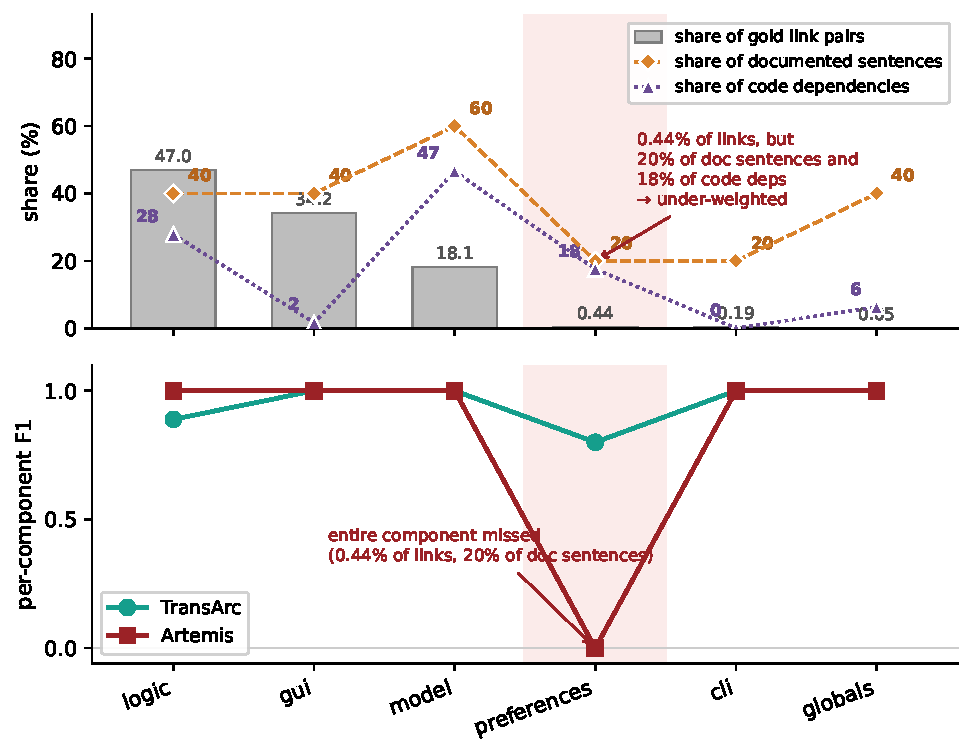
\includegraphics[width=\linewidth]{figures/jabref_motivation_linear}
\caption{JabRef components, ordered by link share. \emph{Top:} small components own
almost none of the doc-code links (grey) although the documentation describes them
(orange) and much of the code depends on them (purple)---two importance axes the
link-level metric ignores. \emph{Bottom:} per-component \fone\ for \TransArc{} and
\Artemis{} (mean of three GPT-5.6-terra runs); \Artemis{} is weakest precisely on
\texttt{preferences}, the component that owns $0.44\%$ of the links.}
\Description{A two-panel chart for JabRef component importance.
The top panel shows that three large components dominate the number of doc-code links
while small components contribute almost none, yet documentation sentence share and
code-dependency share are spread much more evenly across all six components.
The bottom panel plots per-component F1 for TransArc and Artemis, showing that Artemis
scores lowest on the small preferences component, which the link-weighted average hides.}
\label{fig:motivation}
\end{figure}

%SPEC [ev-tools] role: ground in the Artemis/TransArc contrast; minimum figures needed.
%NOTE [arm] (2026-08-28) \Artemis{} here is the GPT-5.6-terra re-run, mean of 3 -- the same
%  system sec:results reports, so the two sections describe one tool. The released gpt-5.4 arm
%  scored 0.998 on JabRef and exactly 0 on preferences, which made the ranking inversion
%  visible inside JabRef alone; the re-run scores 0.916 on JabRef, BELOW TransArc's 0.943, so
%  that single-project version of the claim is gone. The inversion is now stated over the
%  benchmark, where it still holds (+1.0pp link-level, -4.7pp worst, -4.1pp harmonic).
The long-tailed distribution affects published tools.
On JabRef, \Artemis{} is weakest on exactly this component: it scores $0.53$ on \texttt{preferences} against \TransArc{}'s $0.800$, and abandons it outright in one run of three (\autoref{fig:motivation}, bottom).
Its \fone\ on the three large components stays near $0.9$, so the link-level average barely registers the hole---\texttt{preferences} carries $0.44\%$ of the links.
Across the benchmark this inverts the ranking: \Artemis{} leads \TransArc{} by $1.0$pp of link-level \fone\ while trailing it by $4.7$pp on the worst component and $4.1$pp on the harmonic mean.
Link-level \fone{} therefore ranks the tool that covers less of the architecture above the one that covers more.
Weighting recall twice as heavily does not rescue the aggregate: under \ftwo{} \Artemis{}'s link-level lead grows to $6.1$pp while it still trails on the harmonic per-component mean, so what the average hides is not an artifact of balancing precision against recall.
%NOTE [beta] (2026-09-11) the \ftwo{} clause is deliberately scoped to the HARMONIC mean, and
%  the \fone{} inversion sentence above it is deliberately scoped to \fone{}. The full picture
%  from tab:rq2-results.csv (\Artemis{} vs \TransArc{}, pp):
%      link      +1.0 (\fone)   +6.1 (\ftwo)
%      worst     -4.7 (\fone)  +0.95 (\ftwo)   <-- SIGN FLIPS under \ftwo
%      harmonic  -4.1 (\fone)   -0.9 (\ftwo)
%  (worst \ftwo{} is +0.95pp, not +1.0pp: .5243 - .5148 = .0095. Quote it as 0.95 or as
%  "under a point"; rounding it to 1.0 invites a reviewer to recompute and find 0.9.)
%  So the worst-component half of the inversion is \fone-only: \Artemis{} .5243 vs \TransArc{}
%  .5148 on worst \ftwo{}. Do NOT write "the inversion holds under both betas" -- it does not.
%  What IS beta-robust is the SWING between the link level and the tail (5.1pp at beta=1,
%  7.0pp at beta=2), which is the claim the sentence above makes. discussion.tex:22 already
%  explains the mechanism: the backend re-run buys \Artemis{} recall and costs it precision,
%  which is exactly why its \ftwo{} reads better than its \fone{} everywhere.
%REBASED [ev-docmodel] (2026-09-11) this parked block was written against s92a and its
%  \approach{} numbers were STALE: it said \approach{} abandons one component at macro \cmr{}
%  $1.9\%$, but the reported s110 arm abandons NONE at $0.0\%$ (tab:rq2-results.csv, and
%  intro.tex:44 + the RQ2 answer both now claim $0.0\%$). Numbers below re-read off the
%  current table so the block is safe to revive; the baselines never moved in the arm swap.
% %SPEC [ev-docmodel] role: separate the doc-model consequence; show the same silent-failure principle without conflating task granularity.
% The same principle reappears on the doc-model task.
% A system can score well on link-level \fone\ yet abandon a documented component's
% sentences entirely.
% We measure that abandonment directly with the \cmrname{} (\cmr) of \autoref{sec:metric:suite}.
% On doc-model, \approach{} abandons no documented component in any run (macro \cmr{} $0.0\%$).
% \Artemis{} abandons two per run and SWATTR three (macro \cmr{} $3.3\%$ and $7.1\%$).
% \Artemis{} abandons the \texttt{preferences} component on JabRef, the very component this section highlights.
% SWATTR drops three MediaStore components.
%SPEC [ev-close] role: close with the paper move; introduce size-aware metrics that expose dropped components.
This motivates us to quantify the long-tailed distribution across all five projects and introduce size-aware metrics
that expose dropped components.
